\competentie
{% competentieformulier
	\competentieformulier
	{% toelichting
		You are able to reflect on your own performance and to identify your own strengths and weaknesses. You are receptive to other people's views and feedback and use them to grow as an ICT professional.
	}
	{% deelcompetenties
		reflection,%
		self-management%
	}
	{%
		Proof
	}
	{%
		reflection
	}
	{% verwijzing naar bewijs
		Figure~\ref{fig:terraform}
		Figure~\ref{fig:react}
		Figure~\ref{fig:kubernets},
		\ref{fig:vim}
	}
}
{% bewijzen
	\bewijs
	{
		Apply new knowledge
	}
	{% starr
		\starr
		{% betreft
			self-management
		}
		{% datum
			22-05-22
		}
		{% situatie
			It's always easy to take the easy route, use technologies which you are already familiar with.
			This however could lead to a stagnation in skills.

			I want to force myself to apply the new knowledge learned from the cursusses and build a production ready application.
		}
		{% taak
			Study the content and understand the content of the curssuses so I can apply it in a real life scenario.
		}
		{% activiteiten
			Study the matrial and apply it.

		}
		{% resultaat
			The result was a lot of trying and failing and even coming to the conclusion that some technologies aren't even able to be used(terraform).

			But I learned a lot and everything I learned is appliable in my current work environment.

		}
		{% reflectie
			It's not always easy to learn knew technologies when the old still suffice.
			But with learning the new tech I'm able to be more creative with future solutions as it unlocks a whole new stack.

			For example terraform which isn't used in this application but has endless possibilities in an enterprise setting.
			By forcing myself to take some time an learn these new skills i'm able to fullfill my job with more expertice.
		}
		{

		}
	}
	{% bewijs

		Figure~\ref{fig:terraform}

		Figure~\ref{fig:react}

		Figure~\ref{fig:kubernets}
	},
	\bewijs
	{
		Do it well or not at all.
	}
	{% starr
		\starr
		{% betreft
			reflection
		}
		{% datum
			22-05-22
		}
		{% situatie
			I moved from Intellij to Vim for my default editor.
			This lead to mis configuration which then leads to redunancy or mistakes.
		}
		{% taak
			Even when switching editor still maintaine excellent code quality.
		}
		{% activiteiten
			With the new configuration for my Vim I skipped out on configurating lombok.
			Lombok is a tool that generates getters and setters.


			I should have configurated my env in such a way I can still use lombok or delete the packages if i'm not going to use it.

		}
		{% resultaat
			I didn't reconfigure my configuration and still kept the lombok package.
			This lead to a bloat jar file with unnesecary packges.
		}
		{% reflectie
			The whole process of setting up vim for Java development was quit a task.
			For example setting it up for python is straight forward(default langauage used at VanMoof)

			After a lot of tweaking I got it to work and didn't go the extra mile to achieve every feature.

			I should have removed the package or configure it good so it works.
		}
		{
			I can provide my dotfiles or provide access to the repository.
			But only to a single person.

			There are host configrations which I don't want on the WWW.
		}
	}
	{% bewijs
		\label{bewijs:learn}
		Will provide access if mail is provided to Vim configuration.
		\begin{figure}
			\begin{center}
				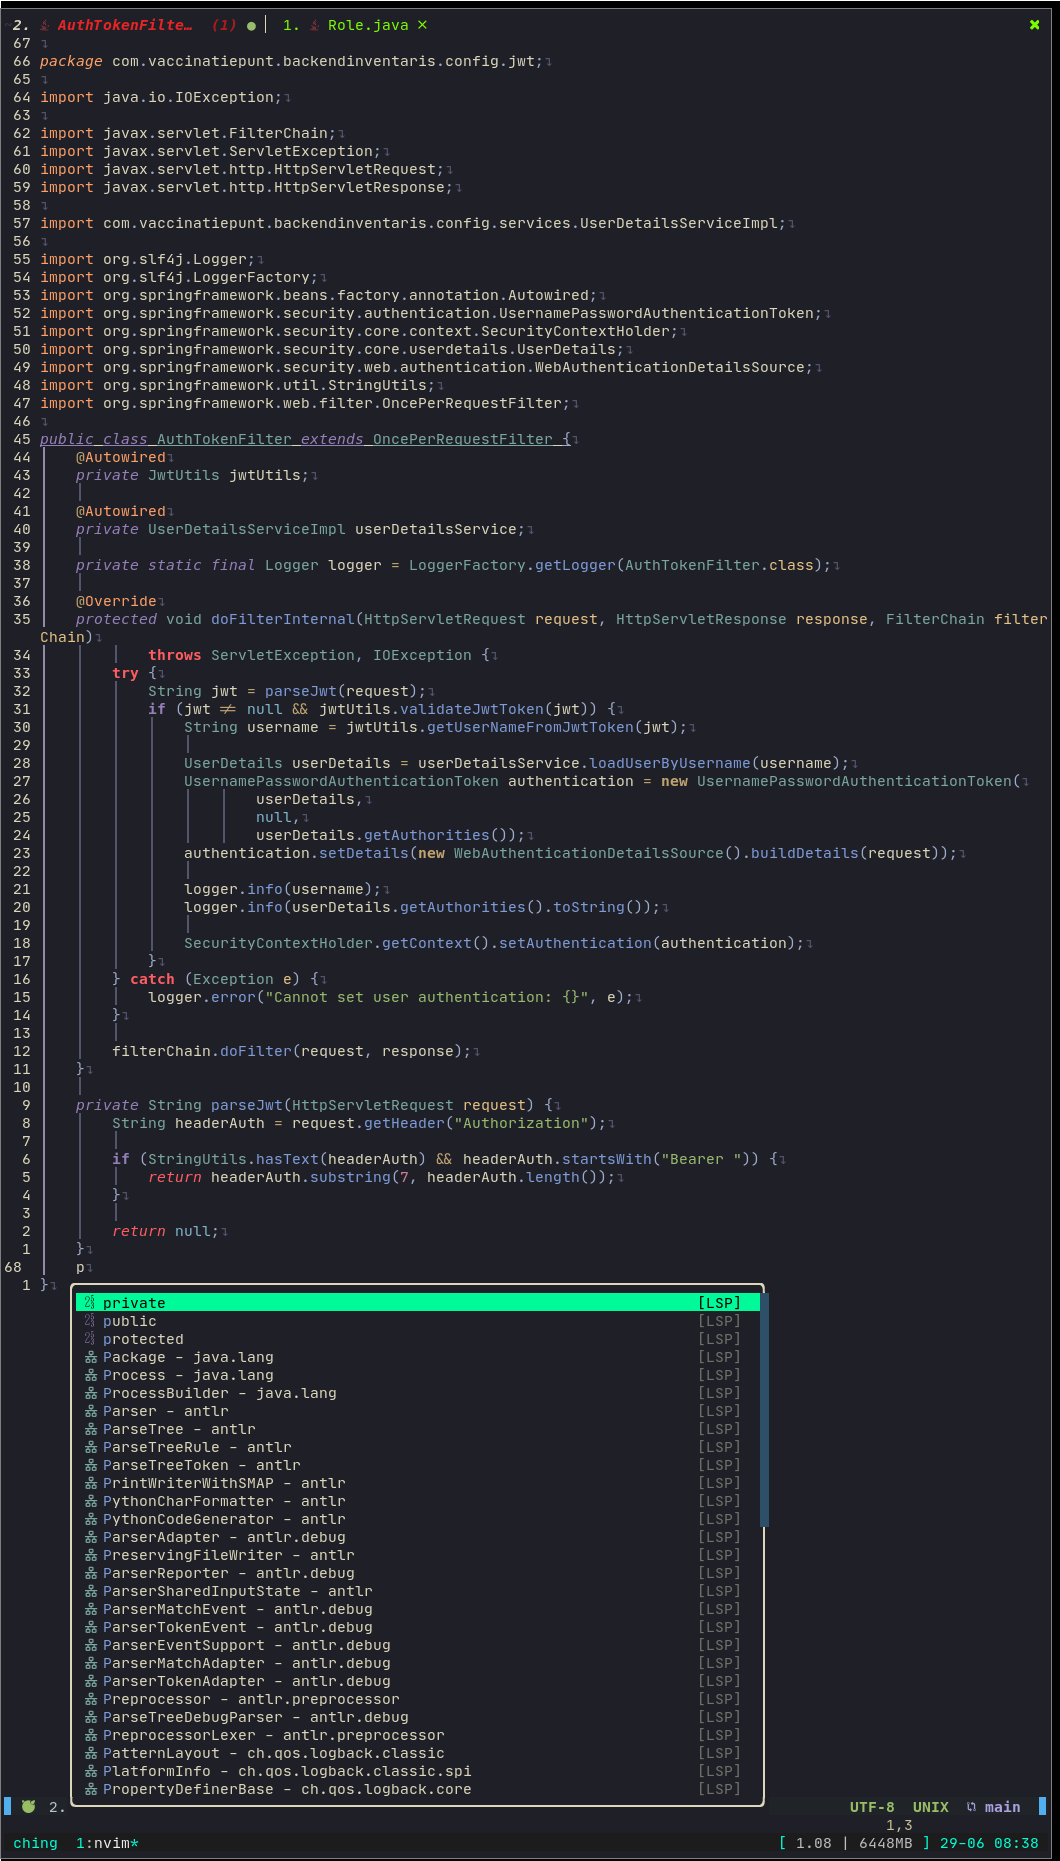
\includegraphics[width=0.95\textwidth]{images/vim.png}
			\end{center}
			\caption{Vim editor development}
			\label{fig:vim}
		\end{figure}

	},
}
